% Version 3 December 2023
% See section 11 of the User Manual for version history
%
%%%%%%%%%%%%%%%%%%%%%%%%%%%%%%%%%%%%%%%%%%%%%%%%%%%%%%%%%%%%%%%%%%%%%%
%%                                                                 %%
%% Please do not use \input{...} to include other tex files.       %%
%% Submit your LaTeX manuscript as one .tex document.              %%
%%                                                                 %%
%% All additional figures and files should be attached             %%
%% separately and not embedded in the \TeX\ document itself.       %%
%%                                                                 %%
%%%%%%%%%%%%%%%%%%%%%%%%%%%%%%%%%%%%%%%%%%%%%%%%%%%%%%%%%%%%%%%%%%%%%

%%\documentclass[referee,sn-basic]{sn-jnl}% referee option is meant for double line spacing

%%=======================================================%%
%% to print line numbers in the margin use lineno option %%
%%=======================================================%%

%%\documentclass[lineno,sn-basic]{sn-jnl}% Basic Springer Nature Reference Style/Chemistry Reference Style

%%======================================================%%
%% to compile with pdflatex/xelatex use pdflatex option %%
%%======================================================%%

%%\documentclass[pdflatex,sn-basic]{sn-jnl}% Basic Springer Nature Reference Style/Chemistry Reference Style

%%Note: the following reference styles support Namedate and Numbered referencing. By default the style follows the most common style. To switch between the options you can add or remove “Numbered” in the optional parenthesis.\\

%%The option is available for: sn-basic.bst, sn-vancouver.bst, sn-chicago.bst%

%%\documentclass[pdflatex,sn-nature]{sn-jnl}% Style for submissions to Nature Portfolio journals
%%\documentclass[pdflatex,sn-basic]{sn-jnl}% Basic Springer Nature Reference Style/Chemistry Reference Style
\documentclass[pdflatex, sn-mathphys-num, lineno]{sn-jnl}% Math and Physical Sciences Numbered Reference Style
%%\documentclass[pdflatex,sn-mathphys-ay]{sn-jnl}% Math and Physical Sciences Author Year Reference Style
%%\documentclass[pdflatex,sn-aps]{sn-jnl}% American Physical Society (APS) Reference Style
%%\documentclass[pdflatex,sn-vancouver,Numbered]{sn-jnl}% Vancouver Reference Style
%%\documentclass[pdflatex,sn-apa]{sn-jnl}% APA Reference Style
%%\documentclass[pdflatex,sn-chicago]{sn-jnl}% Chicago-based Humanities Reference Style

%%%% Standard Packages
%% additional latex packages if required can be included here>
\usepackage{graphicx}%
\usepackage{multirow}%
\usepackage{amsmath,amssymb,amsfonts}%
\usepackage{amsthm}%
\usepackage{mathrsfs}%
\usepackage[title]{appendix}%
\usepackage{xcolor}%
\usepackage{textcomp}%
\usepackage{manyfoot}%
\usepackage{booktabs}%
\usepackage{algorithm}%
\usepackage{algorithmicx}%
\usepackage{algpseudocode}%
\usepackage{listings}%

\usepackage{xspace}
\usepackage{standalone}

%% my package start

% for collabration and will remove before submit
\newcommand{\yy}[1]{\textcolor{cyan}{\textbf{[Yangyang: #1]}}}
\newcommand{\rd}[1]{\textcolor{green}{\textbf{[Dr.Yang: #1]}}}
\newcommand{\ty}[1]{\textcolor{orange}{\textbf{[Tingyou: #1]}}}
\newcommand{\qx}[1]{\textcolor{purple}{\textbf{[Qingxiang: #1]}}}

% for collabration and will remove before submit

\usepackage[detect-all=true]{siunitx}
\sisetup{
    scientific-notation=false,
    round-mode = places,
    round-precision = 2
}

\usepackage[acronym, automake, style=index, shortcuts]{glossaries-extra}

\setabbreviationstyle[acronym]{long-short}

% define glossaries
\makeglossaries
\newacronym{blat}{BLAT}{BLAST-like alignment tool}
\newacronym{llm}{LLM}{Large Language Model}
\newacronym{hmm}{HMM}{Hidden Markov Model}
\newacronym{gpu}{GPU}{Graphics Processing Unit}
\newacronym{hpc}{HPC}{High Performance Computing}
\newacronym{bert}{BERT}{Bidirectional Encoder Representations from Transformers}
\newacronym{gpt}{GPT}{Generative Pre-trained Transformer}

\newacronym{ide}{IDE}{Integrated Development Environment}
\newacronym{cd}{CD}{Continuous Development}
\newacronym{ucsc}{UCSC}{UCSC Genome Browser}
\newacronym{glm}{GLM}{Genomic Language Model}
\newacronym{lcglm}{LCGLM}{long-context genomic language model}
\newacronym{snp}{SNP}{Single Nucleotide Polymorphism}
\newacronym{fm}{FM}{Foundational Model}
\newacronym{nlp}{NLP}{Natural Language Processing}

\newacronym{mlp}{MLP}{multilayer perceptron}
\newacronym{drs}{DRS}{direct RNA sequencing}
\newacronym{ont}{ONT}{Oxford Nanopore Technologies}
\newacronym{pb}{PacBio}{Pacific Biosciences}

\newacronym{go}{GO}{Gene Ontology}
\newacronym{r2c2}{R2C2}{Rolling Circle Amplification to Concatemeric Consensus}
\newacronym{pcr}{PCR}{Polymerase Chain Reaction}

\newacronym{tp}{TP}{True Positive}
\newacronym{fp}{FP}{False Positive}
\newacronym{fn}{FN}{False Negative}

\newcommand{\figref}[2]{Fig.~\hyperref[#1]{\ref*{#1}#2}}
\newcommand{\edfigref}[2]{Extended Data Fig.~\hyperref[#1]{\ref*{#1}#2}}
\newcommand{\edfigrefrg}[3]{Extended Data Fig.~\hyperref[#1]{\ref*{#1}#2-\ref*{#1}#3}}
%% my package end


%%%%%=============================================================================%%%%
%%%%  Remarks: This template is provided to aid authors with the preparation
%%%%  of original research articles intended for submission to journals published
%%%%  by Springer Nature. The guidance has been prepared in partnership with
%%%%  production teams to conform to Springer Nature technical requirements.
%%%%  Editorial and presentation requirements differ among journal portfolios and
%%%%  research disciplines. You may find sections in this template are irrelevant
%%%%  to your work and are empowered to omit any such section if allowed by the
%%%%  journal you intend to submit to. The submission guidelines and policies
%%%%  of the journal take precedence. A detailed User Manual is available in the
%%%%  template package for technical guidance.
%%%%%=============================================================================%%%%

%% as per the requirement new theorem styles can be included as shown below
\theoremstyle{thmstyleone}%
\newtheorem{theorem}{Theorem}%  meant for continuous numbers
%%\newtheorem{theorem}{Theorem}[section]% meant for sectionwise numbers
%% optional argument [theorem] produces theorem numbering sequence instead of independent numbers for Proposition
\newtheorem{proposition}[theorem]{Proposition}%
%%\newtheorem{proposition}{Proposition}% to get separate numbers for theorem and proposition etc.

\theoremstyle{thmstyletwo}%
\newtheorem{example}{Example}%
\newtheorem{remark}{Remark}%

\theoremstyle{thmstylethree}%
\newtheorem{definition}{Definition}%

\raggedbottom
\unnumbered% uncomment this for unnumbered level heads

\begin{document}

\title[Article Title]{Language model identify artificial chimeric read in Nanopore direct RNA sequencing data.}

%%=============================================================%%
%% GivenName	-> \fnm{Joergen W.}
%% Particle	-> \spfx{van der} -> surname prefix
%% FamilyName	-> \sur{Ploeg}
%% Suffix	-> \sfx{IV}
%% \author*[1,2]{\fnm{Joergen W.} \spfx{van der} \sur{Ploeg}
%%  \sfx{IV}}\email{iauthor@gmail.com}
%%=============================================================%%

\author[1]{\fnm{Yangyang} \sur{Li}}\email{yangyang.li@northwestern.edu}
\equalcont{These authors contributed equally to this work.}

% \author*[1,2]{\fnm{First} \sur{Author}}\email{iauthor@gmail.com}
\author[1]{\fnm{Tingyou} \sur{Wang}}\email{tywang@northwestern.edu}
\equalcont{These authors contributed equally to this work.}

\author[1]{\fnm{Qingxiang} \sur{Guo}}\email{qingxiang.guo@northwestern.edu}
\author*[1,2]{\fnm{Rendong} \sur{Yang}}\email{rendong.yang@northwestern.edu}

\affil[1]{\orgdiv{Department of Urology}, \orgname{Northwestern University Feinberg School of Medicine}, \orgaddress{\street{303 E Superior St}, \city{Chicago}, \postcode{60611}, \state{IL}, \country{USA}}}
\affil[2]{\orgdiv{Robert H. Lurie Comprehensive Cancer Center}, \orgname{Northwestern University Feinberg School of Medicine}, \orgaddress{\street{675 N St Clair St}, \city{Chicago}, \postcode{60611}, \state{IL}, \country{USA}}}

% \author[1,2]{\fnm{Third} \sur{Author}}\email{iiiauthor@gmail.com}
% \equalcont{These authors contributed equally to this work.}

% \affil*[1]{\orgdiv{Department}, \orgname{Organization}, \orgaddress{\street{Street}, \city{City}, \postcode{100190}, \state{State}, \country{Country}}}
% \affil[2]{\orgdiv{Department}, \orgname{Organization}, \orgaddress{\street{Street}, \city{City}, \postcode{10587}, \state{State}, \country{Country}}}
% \affil[3]{\orgdiv{Department}, \orgname{Organization}, \orgaddress{\street{Street}, \city{City}, \postcode{610101}, \state{State}, \country{Country}}}

%%==================================%%
%% Sample for unstructured abstract %%
%%==================================%%

\abstract{
    The accurate identification of chimeric reads is critical for ensuring the reliability of nanopore \gls{drs} data, which has emerged as a powerful tool for sequencing full-length RNA molecules while preserving native RNA modifications. Despite its potential, nanopore \gls{drs} is susceptible to the generation of chimeric reads, where fragments of distinct RNA molecules are incorrectly joined together, complicating downstream analyses such as transcriptome assembly and gene fusion detection.

    In this study, we present DeepChopper, a genomics language model specifically designed to detect and filter chimeric reads. Leveraging advanced long-range attention mechanisms and tailored tokenization strategies, DeepChopper effectively distinguishes true biological sequences from artificial constructs with high precision. We validated the performance of DeepChopper across multiple datasets, including \gls{ont} \gls{pcr} cDNA, \gls{ont} CapTrap-seq, \gls{ont} \gls{r2c2}, \gls{pb} cDNA, and \gls{pb} CapTrap-seq.

    Our results demonstrate that DeepChopper significantly outperforms existing methods, achieving up to a 94\% reduction in unsupported reads and consistently maintaining high support rates across diverse sequencing platforms. Additionally, DeepChopper effectively identified low-quality artificial sequences based on base quality scores and \gls{blat} identity, further enhancing the accuracy of nanopore \gls{drs} data.

    This study highlights the potential of DeepChopper to improve the integrity of nanopore \gls{drs} data, paving the way for more reliable genomic analyses and broadening the applicability of genomics language models in bioinformatics.}

\maketitle
\section{Main}\label{sec1}

% Outline
% 1. Sequencing history
% 2. Genomics LLM history
% 3. Challenges of LLM / efficiency of transformer and improvements (hyena)
% 3.1 long range
% 3.2 single nucleotide resolution
% 4. Cons of drs
% 5. Our method
% 6. Results
% 7. Conclusion

The advent of high-throughput sequencing technologies has revolutionized genomics, providing unprecedented insights into the genetic underpinnings of biological processes.
Nanopore \gls{drs} has emerged as a powerful tool for sequencing full-length RNA molecules, preserving native RNA modifications~\cite{ozsolak2009direct, garalde2018highly, jain2022advances}.
However, this technology faces a significant challenge: the generation of artificial chimeric reads where fragments of distinct RNA molecules are incorrectly joined together~\cite{smith2020molecular}.
Accurately identifying these chimeric sequences is critical for maintaining data quality and ensuring reliable downstream analyses, including transcriptome assembly, quantification, and gene fusion detection.

Traditional methods for identifying chimeric reads often struggle with the intricacies of long RNA sequences, leading to errors and inefficiencies.
While recent advances in \gls{llm} have shown promise in genomics, their application to long-read sequencing data remains challenging due to the need for modeling long-range dependencies and achieving single-nucleotide resolution~\cite{dalla2023nucleotide, tay2022efficient, zhou2023dnabert2}.
To address these limitations, we developed DeepChopper, a novel language model specifically tailored for biological sequences.
DeepChopper introduces a hybrid architecture that combines a \gls{lcglm} HyenaDNA for efficient long-range dependency modeling with residual block and \gls{mlp} for fine-grained sequence analysis, achieving both broad context understanding and single-nucleotide resolution~\cite{poli2023hyena, nguyen2024hyenadna, he2016deep} (\figref{fig:f1}{a}).
Uniquely, DeepChopper incorporates base quality information alongside sequence data, enabling more nuanced predictions that account for sequencing confidence.
This quality-aware processing is complemented by an adaptive tokenization strategy that preserves single-nucleotide resolution while capturing higher-order sequence patterns.

A key innovation of DeepChopper is its ability to excel at identifying chimeric reads formed by artificial sequences located in the middle of reads (internal adapters), a capability beyond traditional hard clipping methods that focus only on artificial sequences located in the end of reads (terminal adapters).
By treating biological sequences as a form of language, DeepChopper captures the underlying biological grammar to predict artificial sequences embedded within long reads.
Our approach builds upon recent advancements in \gls{glm} architectures, optimizing for the specific challenges of genomic data processing~\cite{nguyen2024hyenadna}.

Here, we present DeepChopper's performance in accurately identifying artificial chimeric reads in nanopore \gls{drs} data across various library preparation methods and cell lines.
We demonstrate significant improvements over existing methods, particularly in handling the length and variability inherent in RNA sequences.
These results demonstrate the ability of DeepChopper to significantly improve the quality of \gls{drs} data, enabling more accurate and reliable downstream analyses, such as quantification and gene fusion detection.
This work paves the way for broader adoption of \glspl{llm} in enhancing the accuracy and efficiency of biological sequence analysis, ultimately leading to a deeper understanding of the complexities of the transcriptome.


% Result
\begin{figure}[!h]
    \includegraphics[height=0.78\columnwidth]{figures/finals/figure1}
    \caption{{\bf  Detection and analysis of chimeric reads in nanopre \gls{drs} data using DeepChopper.} (a) Overview of the DeepChopper model architecture. Created with BioRender.com (b) Length distribution of predicted artifacts in the VCaP 002 dataset. (c)  Relative positions of prediction artifacts within the VCaP 002 dataset. (d) Number of prediction intervals per read in the VCaP 002 dataset. (e) Chimeric read detection of DeepChopper compared to Dorado (with and without trimming) in the VCaP 002 dataset. The purple bars represent chimeric reads unsupported by \gls{ont} \gls{pcr} cDNA, while the red bars indicate chimeric reads supported by \gls{ont} \gls{pcr} cDNA.  (f) Base quality scores of the artificial sequences identified by DeepChopper. Background colors indicate quality levels: green (high), yellow (medium), red (low). (g) \gls{blat} identity analysis of the artificial sequences detected by DeepChopper. (h) Chimeric read detection of DeepChopper compared to Dorado with trimming across multiple samples, including A549, HCT116, HepG2, K562, and MCF7. In each sample, the blue bars represent chimeric reads unsupported by \gls{ont} \gls{pcr} cDNA, while the red bars indicate chimeric reads supported by \gls{ont} \gls{pcr} cDNA. (i)  Supporting read analysis for WTC11, calculated supporting rate using five different datasets: \gls{ont} \gls{pcr} cDNA, \gls{ont} CapTrap-seq, \gls{ont} \gls{r2c2}, \gls{pb} cDNA, and \gls{pb} CapTrap-seq. The blue bars represent chimeric unsupported reads, while the red bars indicate supported chimeric reads}\label{fig:f1}
\end{figure}

% Model Architecture Overview (Fig 1a)
DeepChopper's architecture integrates a HyenaDNA as a feature extractor with advanced tokenization and quality assessment mechanisms, optimizing it for processing long-range dependencies in sequencing data~\cite{nguyen2024hyenadna} (\figref{fig:f1}{a}).
This design enables efficient differentiation between true biological reads and chimeric artifacts in large volumes of genomic data.
% Analysis of Predicted Artifact Lengths Fig 1b
Analysis of predicted artifact lengths in VCaP 002 data (using RNA002 Kit for \gls{drs}) revealed DeepChopper's efficacy in identifying artificial sequences within a critical length range often associated with chimeric reads.
The majority of detected artifacts were approximately 70 bp long, a range where traditional methods typically struggle due to sequence ambiguity (\figref{fig:f1}{b}).
% Positional Bias in Chimeric Read Prediction Fig 1c
Importantly, DeepChopper demonstrated a consistent ability to identify artificial sequences not only at read ends but also embedded within reads (\figref{fig:f1}{c}) which cause artificial chimeric reads.
This capability is crucial for nanopore \gls{drs} data, where artificial chimeric reads can significantly impact downstream analyses~\cite{smith2020molecular}.

% The number of prediction intervals Fig 1d
Analysis of prediction intervals in the VCaP 002 dataset revealed DeepChopper's sensitivity to artificial sequences.
A prediction interval is defined as a contiguous sequence within a read where the model predicts the presence of artificial sequences.
In most cases, DeepChopper predicted a single interval, typically located internally or at the end of the read.
We focused on reads with two or more prediction intervals, as these may indicate artificial chimeric reads.
Most reads contained 1-5 intervals, with multiple intervals potentially indicating fragmented chimeric sequences often missed by Dorado (\figref{fig:f1}{d}).

% Base Quality and BLAT Identity of Artificial Sequences at the End of Reads (Supplementary Fig 1a)
Further validation of DeepChopper's performance came from analyzing base quality and \gls{blat} identity of artificial sequences at read ends in a 1 million read subsample from the VCaP 002 dataset (\edfigref{fig:sf1}{a}).
Terminal artificial sequences showed lower average base quality scores (~10) and \gls{blat} identity values (~0.3), consistent with their characterization as sequencing artifacts or erroneous terminal adapters.
% Comparison of Soft-Clipping Regions to Terminal Adapters Identified by DeepChopper (Supplementary Fig 1b)
Comparison of soft-clipping regions in Dorado-processed data (without trimming) to DeepChopper-identified terminal adapters showed 99.6\% alignment (\edfigref{fig:sf1}{b}).
Of the 0.4\% non-aligned sequences, 97\% failed to map to the reference genome, further confirming their artificial nature.
These results underscore DeepChopper's reliability in identifying artificial sequences, particularly at read ends, demonstrating its potential to enhance data quality in nanopore \gls{drs} analysis.

% Chimeric Read Detection Across Sequencing Platforms Fig 1e
DeepChopper significantly outperformed Dorado in artificial chimeric read detection, achieving a 91\% reduction in total chimeric read count for the VCaP 002 dataset (\figref{fig:f1}{e}).
Validation using \gls{ont} \gls{pcr} cDNA data showed DeepChopper reduced unsupported reads by 94\% and increased the supporting rate from 5\% to 47\%, demonstrating superior accuracy in distinguishing true biological sequences from chimeric constructs (\figref{fig:f1}{e}).
% Base Quality of Detected Artificial Sequences (Fig 1f)
To assess the quality of detected artificial sequences, we analyzed their base quality scores. \figref{fig:f1}{f} specifically shows the base quality of internal artificial sequences in \gls{fp} chimeric reads, which are unique chimeric reads in VCaP 002 data processed by Dorado with trim compared to the same data processed by DeepChopper.
The artificial sequences identified by DeepChopper consistently exhibited lower base quality scores, aligning with the expected profile of erroneous reads.
The result further validates the accuracy of DeepChopper in identifying and filtering out artificial sequences (\figref{fig:f1}{f}).
% BLAT Identity of Detected Artificial Sequences (Fig 1g)
We also evaluated the \gls{blat} identity of internal artificial sequences in \gls{fp} chimeric reads in VCaP 002 data processed by Dorado with trim  (\figref{fig:f1}{g}).
\gls{blat} identity measures the similarity of the sequences to known reference sequences, with lower identity scores indicating potential chimeric or erroneous reads.
The results show that the artificial sequences identified by DeepChopper consistently have lower \gls{blat} identities.
This finding highlights the model's proficiency in detecting sequences that diverge from expected reference sequences, further confirming their artificial nature.

These comprehensive analyses demonstrate DeepChopper's superior performance in identifying and filtering out chimeric reads and artificial sequences in nanopore \gls{drs} data.
By maintaining high precision in detecting lower-quality and divergent sequences, DeepChopper significantly enhances the overall integrity of sequencing data, ensuring that downstream analyses are based on more accurate and reliable reads.

% Performance of DeepChopper on VCaP 004 Data (Supplementary Fig 1C and 1D)
To assess the performance of DeepChopper across different protocols, we applied the model to VCaP 004 data, sequenced using the newer RNA004 protocol designed for cleaner data output.
DeepChopper achieved a 21\% reduction in chimeric reads compared to Dorado with trimming, increasing the supporting ratio from 25\% to 30\% when validated against \gls{ont} \gls{pcr} cDNA data (\edfigref{fig:sf1}{c}).
Analysis of \gls{fp} chimeric reads in VCaP 004 showed consistently low base quality scores (averaging around 10) and \gls{blat} identity (clustering around 0.3) for artificial sequences (\edfigref{fig:sf1}{d}).
These results, mirroring those from VCaP 002, demonstrate DeepChopper's robustness in identifying chimeric artifacts across different \gls{drs} protocols.

% Chimeric Read Detection Across Multiple Samples (Fig 1h)
To demonstrate DeepChopper's broad applicability  and effectiveness, we extended our analysis to multiple samples and sequencing platforms.
Across five different cell lines (A549, HCT116, HepG2, K562, and MCF7) using the RNA002 protocol for \gls{drs}, DeepChopper consistently reduced chimeric reads by 62-84\% compared to baseline methods (\figref{fig:f1}{h}).
The supporting rate improved from 8-19\% (Dorado with trimming) to 43-55\% (DeepChopper), mirroring the performance observed in the VCaP 002 dataset (\figref{fig:f1}{e}).
This consistent performance across diverse samples underscores DeepChopper's robustness and reliability in various cell lines.

% Supporting Read Analysis Across Multiple Datasets (Fig 1i)
We further validated DeepChopper's effectiveness using the WTC11 sample, leveraging multiple sequencing platforms to verify chimeric read detection (\figref{fig:f1}{i}).
DeepChopper reduced chimeric reads in WTC11 by 54\% compared to Dorado with trim.
To assess the accuracy of chimeric read identification, we calculated supporting read rates using data from five different platforms: \gls{ont} \gls{pcr} cDNA, \gls{ont} CapTrap-seq, \gls{ont} \gls{r2c2}, \gls{pb} cDNA, and \gls{pb} CapTrap-seq~\cite{carbonell2024captrap}.
DeepChopper consistently achieved high support rates (51-66\%) across these diverse datasets, compared to 26-37\% for Dorado with trimming.
This cross-platform validation demonstrates DeepChopper's versatility and accuracy in maintaining data integrity across various sequencing conditions.

These comprehensive analyses collectively showcase DeepChopper's superior performance in detecting and filtering artificial chimeric reads.
The consistency of results across diverse datasets reinforces DeepChopper's reliability in enhancing the quality of nanopore \gls{drs} data, providing a robust solution for improving the accuracy of downstream genomic analyses.

\begin{figure}[!h]
    \includegraphics[height=1.2\columnwidth]{figures/finals/figure2}
    \caption{\bf This is figure 2.}\label{fig:f2}
\end{figure}

% Comparison of Gene Expression Levels Between Reference and FP Genes (Fig 2a)
In the VCaP 002, genes in the \gls{fp} group exhibited significantly higher expression levels compared to reference genes (\(\textrm{p-value} < 2.2 \times 10^{-16}\)) (\figref{fig:f2}{a}), despite displaying similar gene lengths (\figref{fig:f2}{b}).
This result suggests that the \gls{fp} genes detected by DeepChopper, after comparing with Dorado, are characterized by higher expression levels, which may indicate their association with artificial sequences or chimeric reads rather than true biological signals.
This pattern highlights the effectiveness of DeepChopper in distinguishing between genuine gene expression and artifacts introduced during sequencing, thereby improving the overall accuracy of gene expression analysis in the dataset.

% Visualization of Chromosomal Connections in FP Chimeric Reads (Supplementary Fig 2a)
To investigate potential patterns among \gls{fp} chimeric reads, we visualized the chromosomal regions connected by all \gls{fp} chimeric reads from the VCaP 002 dataset (\edfigref{fig:sf2}{a}).
This analysis aimed to detect any recurring connections between specific genomic regions that might indicate systematic artifacts in the sequencing data.
The results did not reveal any clear or consistent patterns of chromosomal connections in the \gls{fp} chimeric reads.s
The connections appeared to be randomly distributed across various chromosomes, with no particular region showing a higher frequency of connections (\edfigref{fig:sf2}{a}).
This lack of an obvious pattern suggests that the occurrence may not be driven by specific genomic locations but rather by random sequencing or data processing errors.
These findings imply that \gls{fp} chimeric reads are likely due to non-specific factors rather than biases associated with particular chromosomal regions, underscoring the need for robust detection and filtering methods, such as those provided by DeepChopper, to improve data quality.

% Gene Ontology (GO) Enrichment Analysis of FP Group Genes (Fig 2c)
To further explore the functional roles of the \gls{fp} group genes, we conducted a \gls{go} enrichment analysis across six cell lines: VCaP, A549, K562, HepG2, MCF7, and HCT116 (\edfigrefrg{fig:sf2}{b}{g}).
We illustrate the overlapping \gls{go} pathways enriched among the \gls{fp} genes across these cell lines (\figref{fig:f2}{c}).
The results show a substantial overlap in \gls{go} terms related to core biological processes, particularly those associated with ribosomal small subunit biogenesis, cytoplasmic translation, translational elongation, and rRNA processing (\figref{fig:f2}{c}).
This overlap indicates that the \gls{fp} group genes are frequently involved in pathways critical to protein synthesis and ribosome function.
Such pathways are typically highly expressed and conserved across different cell types, which might explain their recurrent identification as false positives.
The significant intersection sizes for these \gls{go} terms across the six cell lines suggest a common pattern in the \gls{fp} gene set, reinforcing the hypothesis that these genes might be artifacts associated with sequencing or data processing errors rather than true biological signals.
This finding highlights the need for careful evaluation of \gls{gpt} genes in high-throughput sequencing studies to avoid misleading conclusions about gene function.

Our study demonstrates the potential of large language models in biological sequence analysis, particularly in the context of nanopore \gls{drs}.
By accurately predicting adapter sequences,  \glspl{llm} can significantly improve the quality and reliability of sequencing data.
This showcases the broader applicability of language models in handling complex biological data, paving the way for advancements in genomics and transcriptomics.
Future research can explore additional applications and further optimize these models for specific biological tasks, solidifying their role in biotechnology.


\section{Methods}\label{sec:methods}

\subsection{Cell culture}

VCaP 002 cell lines were obtained from the American Type Culture Collection (ATCC) and cultured under sterile conditions to maintain optimal growth and viability.
The cells were grown in Dulbecco's Modified Eagle Medium (DMEM, high glucose; Gibco, Cat\# 11-965-092) supplemented with 10\% fetal bovine serum (FBS Opti-Gold, Performance Enhanced, US Origin; Gendepot, Cat\# F0900-050) to provide essential growth factors.
In addition, the culture medium was enriched with \SI{5}{\ml} of 100 mM \( 100\times \) Sodium Pyruvate (Gendepot, Cat\# CA017-010) to support cellular metabolism and \SI{5}{\ml} of Antibiotics-Antimycotics (\( 100\times \)) (Gendepot, Cat\# CA002-010) to prevent microbial contamination.
Cells were cultured in \SI{100}{\mm} cell culture treated dishes (Thermo Fisher Scientific, Cat\# 12-556-002) and incubated at \SI{37}{\degreeCelsius} in a humidified atmosphere containing 5\% CO2, with media changes performed every 72 hours to ensure nutrient availability and waste removal.
Cell confluency was regularly monitored, and subculturing was done before reaching 80\% confluency to maintain healthy growth conditions and prevent over-confluence stress.

\subsection{RNA extraction and quantification}

Total RNA was extracted using the miRNeasy Mini Kit (Qiagen, Cat\# 217004) according to the protocol of the manufacturer.
The quality and concentration of RNA were assessed using an Agilent 2100 Bioanalyzer.
Poly(A)+ RNA was then enriched from the total RNA using the Dynabeads\textsuperscript{tm} mRNA Purification Kit (Invitrogen, Cat\# 65001), which utilizes oligo (dT) beads for selective mRNA binding.
The mRNA was quantified using a Qubit 4 fluorometer and a Qubit RNA HS Assay Kit (Thermo Fisher Scientific, Cat\# Q32852).
The mRNA preparations were either immediately used to prepare a sequencing library or frozen and stored at \SI{-80}{\degreeCelsius} until further use.

\subsection{Nanopore sequencing}

We performed nanopore sequencing of the enriched mRNA using two different chemistries: the DNA-nanopore (R9 chemistry; RNA002 kit) and the RNA-nanopore chemistry (RNA chemistry; RNA004 kit).
For the RNA002 library, \SI{1}{\micro\gram} of poly(A)+ RNA was used as input for library preparation using the Direct RNA Sequencing Kit (SQK-RNA002, \gls{ont}) following the manufacturer's instructions.
Nanopore \gls{drs} employs a reverse transcriptase adapter (RTA) that typically binds to the poly(A) tails of messenger RNA (mRNA); subsequently, a sequencing adapter is ligated to the RTA, which guides the mRNA through the nanopore for sequencing.
The prepared library was loaded onto a MinION flow cell (FLO-MIN106) and sequenced for 48 hours using the Oxford Nanopore MinION device.
For the RNA004 library, 300 ng of poly(A)+ RNA was used as input for library preparation using the Direct RNA Sequencing Kit (SQK-RNA004, \gls{ont}) according to the protocol of the manufacturer.
The library was then loaded onto a PromethION RNA Flow Cell (FLO-PRO004RA) and sequenced on the Oxford Nanopore PromethION device for 72 hours.

\subsection{Training data preparation}\label{ssec:data}

We utilized \gls{ont} directRNA FAST5 data from the SG-Nex project, encompassing six cell lines (HEK293T, A549, K562, HepG2, MCF7, and HCT116)~\cite{chen2021systematic}.
FASTQ files were generated using Dorado (v0.5.2) with adapter trimming disabled (--no-trim) and  model “rna002\_70bps\_hac@v3”.~\cite{dorado2023}.
Reads were aligned to the human reference genome (GRCh38) using minimap2 (v2.24) with optimized \gls{ont} directRNA parameters (-ax splice -uf -k14)~\cite{li2018minimap2}.
For adapter extraction, we selected primary alignments lacking supplementary alignments, treating 3' soft-clipped regions as adapter sequences and aligned portions as non-adapter sequences.

To create artificial chimeric reads, we randomly combined two non-adapter sequences with one adapter sequence.
The resulting SAM files were converted to BAM format, indexed, and sorted using SAMtools (v1.16) to obtain the genome coverage distribution~\cite{li2009sequence}.
Our dataset comprises both positive (terminal and internal adapters in a 1:1 ratio) and negative examples (no artificial sequences) in a 9:1 ratio.
We generated 600,000 data points, split into training (480,000), validation (60,000), and test (60,000) sets with a ratio of 0.8:0.1:0.1.


\subsection{Language model architecture}\label{ssec:lm}

DeepChopper approaches artificial sequence detection as a token classification task, predicting whether each token belongs to an artificial sequence.
The model's architecture is specifically designed for this purpose, enabling accurate identification of artificial sequence regions within biological data.

At its core, DeepChopper adapts the HyenaDNA framework, a genomic model architecture, as its primary feature extractor~\cite{nguyen2024hyenadna}.
This choice enhances the model's ability to process and interpret complex biological sequences effectively.
Following feature extraction, we integrated a quality block to incorporate sequence quality information into the prediction process.
This block, comprising dense layers with residual connections, combines quality scores with extracted features, enriching the model's understanding of the input data.

The integrated features are then passed to a classification head, which outputs the probability of each token being part of an artificial sequence.
This architecture allows DeepChopper to leverage contextual information within biological sequences, ensuring high accuracy in artificial sequence prediction.
By classifying tokens into positive (part of an artificial sequence) or negative (not part of an artificial sequence) categories, DeepChopper provides a nuanced analysis of the input data, crucial for maintaining the integrity of nanopore \gls{drs}  results.


\subsection{Model training}\label{ssec:training}

\textit{Sequence tokenization.} We used a tokenization strategy that converted the biological sequences into single-nucleotide tokens.
The tokens contain \emph{A}, \emph{C}, \emph{G}, \emph{T} and \emph{N} as the basic units, allowing the model to capture the fine-grained details of the sequences.
The model was trained using supervised learning, with sequences annotated for artificial sequences.
Training was conducted on a high-performance computing cluster using two A100 \glspl{gpu}.
The batch size was \num{64}, validation was performed every \num{20000} steps, and we selected the model with the highest validation F1 score for the base prediction task.
The Adam optimizer was used for training with default \( \beta_{1} = 0.9 \) and \( \beta_{2} = 0.999 \) parameters~\cite{kingma2014adam}.
We use a learning rate scheduler to reduce the learning rate when the validation loss stops improving, and the initial learning rate is \num{0.00002}.

Cross-entropy loss was used to update the model parameters:

\[
	\ell(x, y) = L = \{l_1,\cdots,l_N\}^\top, \quad
	l_n = - w_{y_n} \log \frac{\exp(x_{n,y_n})}{\sum_{c=1}^C \exp(x_{n,c})}
	\cdot 1\{y_n \not= \textrm{ignore\_index}\}
\]

where \( x \) is the input, \( y \) is the target, \( w \) is the weight,
\( C \) is the number of classes, and \( N \) spans the minibatch dimension as well as
\( d_1, \cdots, d_k \) for the K-dimensional case.

\[
	\ell(x, y) =   \sum_{n=1}^N \frac{1}{\sum_{n=1}^N w_{y_n} \cdot 1\{y_n \not= \textrm{ignore\_index}\}} l_n
	.\]

Training was conducted for \num{60} epochs with early stopping based on validation performance to prevent overfitting.

Evaluation metrics included accuracy, precision, recall, and F1 score with the following equations:
\begin{align*}
	\textrm{Precision} & = \frac{\textrm{TP}}{\textrm{TP}+\textrm{FP}}                                                     \\
	\textrm{Recall}    & = \frac{\textrm{TP}}{\textrm{TP}+\textrm{FN}}                                                     \\
	\textrm{F1}        & = 2 \times \frac{\textrm{Precision} \times \textrm{Recall}}{\textrm{Precision} + \textrm{Recall}}
\end{align*}

The final model was selected based on the best performance on the validation set.
We use Hydra to find the optimal model's parameters~\cite{Yadan2019Hydra}.
The total loss for one window is the sum of the losses from each supported position.
For per position  \( i \), where \( i  \in {1, 2, \cdots, S} \),  the total loss includes both base prediction loss.
The binary cross-entropy losses were used for these tasks, with the total loss incorporating predicted base probabilities, true base values, and the probability that a position is informative.
The complete list of hyperparameters can be found in Supplementary Table~\ref{tab:hyperparameter}.

\subsection{Polishing predictions with sliding window}

To enhance the accuracy and smoothness of the predictions, we implemented a sliding window approach.
This technique helps to extend the prediction regions and reduces choppy noise, aligning with the typical distribution of artificial sequences in nanopore \gls{drs} data.
The sliding window technique is particularly effective in maintaining continuity in regions where artificial sequences are predicted, ensuring that isolated predictions do not create fragmented and unrealistic results.

We employed a sliding window of size 21 nucleotides.
This window size was chosen based on empirical testing to balance the need for sufficient smoothing while retaining sensitivity to shorter artificial sequences.

Within each sliding window, we applied a voting method to polish the predictions.
The final classification of each nucleotide within the window is determined by the majority vote of all predictions within that window.
The voting result for each nucleotide \( x_i \) is given by:
\[
y_i = \begin{cases}
    1 & \text{if } \sum_{j=i-k}^{i+k} p_j > \frac{W}{2} \\
    0 & \text{otherwise}
\end{cases}
\]
where \( y_i \) is the final prediction for nucleotide \( x_i \). \( p_j \) is the predicted probability of being an artificial sequence for nucleotide \( x_j \). \( W \) is the size of the sliding window, \( k \) is half the window size, i.e., \( k = \frac{W-1}{2} \).


After polishing the predictions using the sliding window, we performed additional filtering to refine the output.
Predicted regions with lengths less than 20 nucleotides were removed, as such short regions are likely to represent noise rather than true artificial sequences.
The remaining sequences, along with their associated quality scores, were then outputted to FASTQ records for further analysis.
This post-processing step ensures that the final output is both accurate and biologically relevant.

The use of sliding windows and the voting method significantly improved the quality of the predictions by smoothing the output and reducing false positives.
By combining these techniques, we were able to produce more reliable predictions, which are crucial for downstream applications such as sequence assembly and variant calling.


\subsection{Evaluating artificial sequences detection}

\textit{Evaluation metrics and analysis.} We assessed DeepChopper's performance using precision, recall, and F1 score, based on \gls{tp} and \gls{fn} counts.
These metrics provided a comprehensive view of the model's ability to identify artificial sequences.
To evaluate DeepChopper's effectiveness across diverse datasets, we analyzed its performance on multiple cell lines (VCaP 002, A549, HCT116, K562, MCF7) and compared it to baseline methods, including Dorado with and without trimming.
We quantified the reduction in chimeric reads and the improvement in supporting rates across these datasets.

We further validated DeepChopper's robustness using cross-platform analysis.
Using the WTC11 cell lines, we calculated supporting read rates using data from five different sequencing platforms: ONT PCR cDNA, ONT CapTrap-seq, ONT R2C2, PacBio cDNA, and PacBio CapTrap-seq.
This cross-platform validation assessed DeepChopper's ability to maintain high support rates across diverse sequencing conditions.
To evaluate the quality of detected artificial sequences, we analyzed their base quality scores and BLAT identity.
We compared these metrics for artificial sequences detected in false positive chimeric reads unique to Dorado processing versus DeepChopper processing.
Statistical analysis, including paired t-tests, was conducted to determine the significance of improvements over traditional methods.
The model's generalizability was further validated by testing on independent datasets, including the VCaP 004 dataset sequenced using the newer RNA004 protocol, demonstrating DeepChopper's adaptability to evolving sequencing technologies.

\textit{Evaluation of artificial chimeric reads in real data.} To evaluate DeepChopper on real data, we used the VCaP 002 dataset, focusing on identifying chimeric reads caused by internal adapters in nanopore DRS data.
We cross-referenced the identified reads with data from multiple sequencing platforms: ONT PCR cDNA, ONT CapTrap-seq, ONT R2C2, PacBio cDNA, and PacBio CapTrap-seq.
Supporting rates, defined as the ratio of chimeric reads corroborated by other platforms to the total detected chimeric reads, were calculated to assess detection consistency across platforms.
We extended our evaluation to multiple cell lines (A549, HCT116, HepG2, K562, MCF7) and the wtc11 cell lines to demonstrate DeepChopper's broad applicability.
This cross-sample and cross-platform validation approach allowed us to assess the model's performance across diverse sequencing contexts.


\textit{BLAT Identity Calculation.} To assess the accuracy of artificial sequences in chimeric read, we calculated the \gls{blat} identity for each sequence using both \gls{blat} and PxBLAT tools.
The BLAT identity is defined as the ratio of the match length to the sequence length, providing a measure of how closely a sequence aligns to a reference genome.
\[
\textrm{BLAT Identity} = \frac{\textrm{Match Length}}{\textrm{Sequence Length}}
\]
Here, the match length refers to the total number of aligned bases that match the reference genome, and the sequence length is the total length of the query sequence.

We aligned the sequences whose length was larger than 20 bp to the reference genome using BLAT (v0.37.2) and PxBLAT (v1.2.1)~\cite{kent2002blat, li2024pxblat}.
The resulting BLAT identity scores were analyzed to differentiate between true biological sequences and artificial chimeric reads.
Sequences with lower BLAT identity were flagged as potential chimeric reads, contributing to the overall assessment of DeepChopper's performance.


\subsection{Gene expression analysis of FP group of chimeric reads}

To identify the false positive (FP) group of chimeric reads, we began by comparing two datasets: the chimeric reads identified by Dorado and those supported by DeepChopper. The FP group was defined by subtracting the chimeric reads confirmed by DeepChopper from the total chimeric reads identified by Dorado. Following the identification of the FP group, we proceeded to assess gene expression levels specifically associated with these reads using IsoQuant\cite{IsoQuant}


\subsection{\gls{go} analysis}

For each cell line, the top 100 high expressed genes were used for the GO enrichment analysis using the Database for Annotation, Visualization, and Integrated Discovery (DAVID)\cite{david} to elucidate the biological processes they involved.

\subsection{Computing resource}

All computations were performed on a \gls{hpc} server equipped with a 64-core Intel(R) Xeon(R) Gold 6338 CPU and 256 GB of RAM.
The server also featured two NVIDIA A100 GPUs, each with 80 GB of GPU memory, providing substantial computational power for both CPU-intensive tasks and GPU-accelerated deep learning workloads.


% \section{Tables}\label{sec5}

% Tables can be inserted via the normal table and tabular environment. To put
% footnotes inside tables you should use \verb+\footnotetext[]{...}+ tag.
% The footnote appears just below the table itself (refer Tables~\ref{tab1} and \ref{tab2}).
% For the corresponding footnotemark use \verb+\footnotemark[...]+

% \begin{table}[h]
% \caption{Caption text}\label{tab1}%
% \begin{tabular}{@{}llll@{}}
% \toprule
% Column 1 & Column 2  & Column 3 & Column 4\\
% \midrule
% row 1    & data 1   & data 2  & data 3  \\
% row 2    & data 4   & data 5\footnotemark[1]  & data 6  \\
% row 3    & data 7   & data 8  & data 9\footnotemark[2]  \\
% \botrule
% \end{tabular}

% \footnotetext{Source: This is an example of table footnote. This is an example of table footnote.}
% \footnotetext[1]{Example for a first table footnote. This is an example of table footnote.}
% \footnotetext[2]{Example for a second table footnote. This is an example of table footnote.}
% \end{table}

% \begin{table}[h]
% 	\caption{Benchmarking for different models}
% 	\label{tab:bechmark}
% 	\begin{tabular}{@{}
% 			l
% 			S[table-format=1.4e-2] % Formats the F1 column in scientific notation
% 			S[table-format=1.4e-2] % Formats the Loss column in scientific notation
% 			@{}}
% 		\toprule
% 		{Model}             & {F1}                         & {Loss}                         \\ \midrule
% 		CNN                 & 0.9909037351608276           & 0.00302332011051476            \\
% 		Model with Hyena    & 0.9925663471221924           & 0.002182388212531805           \\
% 		Model with Caduceus & \bfseries 0.9977396130561829 & \bfseries 0.000541145505849272 \\ \bottomrule
% 	\end{tabular}
% 	% \footnotetext{Source: This is an example of table footnote. This is an example of table footnote.}
% 	% \footnotetext[1]{Example for a first table footnote. This is an example of table footnote.}
% 	% \footnotetext[2]{Example for a second table footnote. This is an example of table footnote.}
% \end{table}


\bmhead{Data Availability}

The human reference genome GRCh38 was downloaded from \url{http://ftp.1000genomes.ebi.ac.uk/vol1/ftp/technical/reference/GRCh38\_reference\_genome/}.


\bmhead{Code Availability}

DeepChopper (v1.0) is available at GitHub (\url{https://github.com/ylab-hi/DeepChopper}).
The scripts for model training, performance valuation and simulate data generation are available at GitHub (\url{https://github.com/ylab-hi/DeepChopper}).
Both repositories are available under a MIT License.

\bmhead{Acknowledgements}

Acknowledgements are not compulsory. Where included they should be brief. Grant or contribution numbers may be acknowledged.
Please refer to Journal-level guidance for any specific requirements.


\backmatter

\begin{appendices}
    \printglossary[type=\acronymtype, title=Abbreviations]

\end{appendices}


\bibliography{sn-bibliography}% common bib file




\newpage

\section{Extend data}

\renewcommand{\figurename}{Extended Data Fig.}


 \begin{figure}[!h]
     \includegraphics[height=0.65\columnwidth]{figures/finals/sf1}
     \caption{ {\bf Analysis of chimeric reads and artificial sequences in VCaP RNA sequencing data } (a) Base quality and \gls{blat} identity of terminal aritifical sequences for subsampling 1M data in VCaP 002. (b) Softcliping part of Dorado untrimed compared with terminal artifical sequenes for subsampling 1M data in VCaP RNA002. (c) VCaP RNA004 chimeric read summary with cDNA support. (d)Base quality and \gls{blat} identity of VCaP RNA004 internal artificial sequences.}
     \label{fig:sf1}
 \end{figure}


 \begin{figure}[!h]
     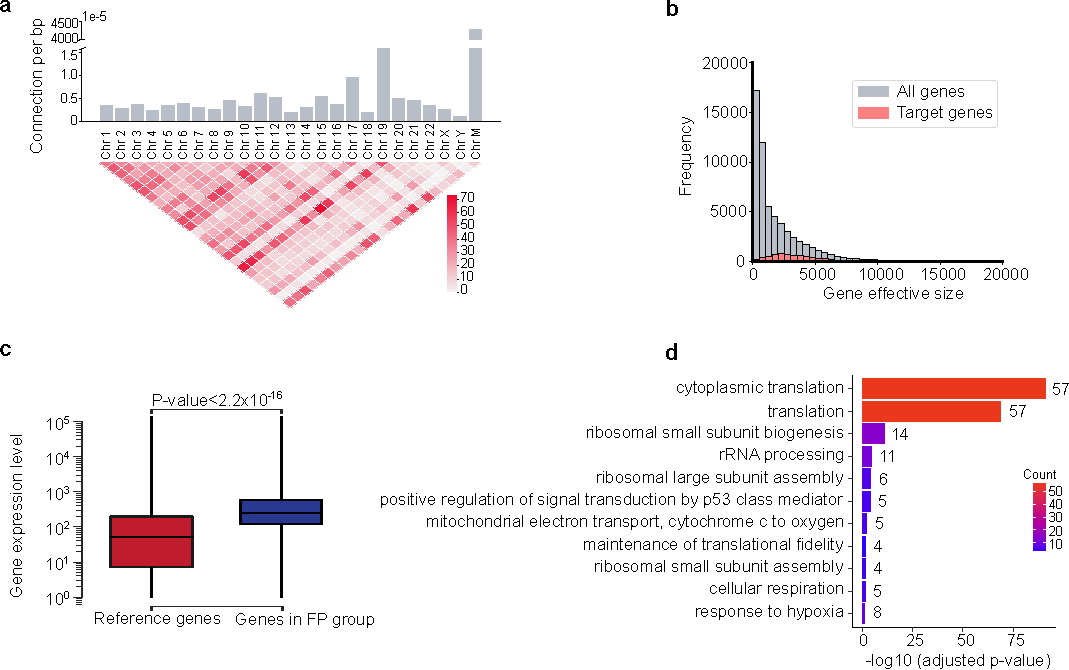
\includegraphics[height=1.2\columnwidth]{figures/finals/sf2}
     \caption{ {\bf  Analysis of \gls{fp} chimeric reads } (a) Visualization of chromosomal connections for all \gls{fp} chimeric reads detected in the VCaP 002 dataset. (b) Distribution of \gls{fp} biological processes enriched among \gls{fp} group genes in A549. (c) Distribution of \gls{fp} biological processes enriched among \gls{fp} group genes in HCT116. (d) Distribution of \gls{fp} biological processes enriched among \gls{fp} group genes in MCF7. (e) Distribution of \gls{fp} biological processes enriched among \gls{fp} group genes in K562. (f) Distribution of \gls{fp} biological processes enriched among \gls{fp} group genes in HepG2. (g) Distribution of \gls{fp} biological processes enriched among \gls{fp} group genes in VCaP.}
     \label{fig:sf2}
 \end{figure}


\newpage

\section{Supplementary information}

\renewcommand{\figurename}{Supplementary Fig.}
\renewcommand{\tablename}{Supplementary Table}


% If your article has accompanying supplementary file/s please state so here.
% Authors reporting data from electrophoretic gels and blots should supply the full unprocessed scans for key as part of their Supplementary information. This may be requested by the editorial team/s if it is missing.
% Please refer to Journal-level guidance for any specific requirements.


\begin{table}
	\centering
	\caption{Hyperparameter ranges used}\label{tab:hyperparameter}
	\begin{tabular}{lc}
		\toprule
		                                    & {$\sf DeepChopper$}                  \\
		\midrule
		Layers                              & 2                                 \\
		Width                               & 256                               \\
		Parameters                          & 1.6M                              \\
		Optimizer                           & AdamW                             \\
		Optimizer momentum                  & $\beta_1$, $\beta_2$ = 0.9, 0.999 \\
		Training epoch                      & 100                               \\
		Batch size                          & 256-1024                          \\
		Learning rate                       & 2e-4 to 1e-3                      \\
		LR scheduler                        & Cosine decay                      \\
		Weight decay (model)                & 0-0.2                             \\
		Weight decay ({$\sf Hyena$} layers) & 0                                 \\
		Embed dropout                       & 0-0.2                             \\
		Residual dropout                    & 0-0.2                             \\
		Sequence lengths                    & 32769                             \\
		\midrule
	\end{tabular}

\end{table}


\begin{table}
    \caption{Open source libraries (and corresponding licenses) used in this work.}
    \label{tab:assets}
            \begin{tabular}{ll}
                \toprule
                Library                                                & License                                                                            \\ \midrule
                GenomicsBenchmark~\cite{grevsova2023genomic}           & Apache 2.0                                                                         \\
                Mamba~\cite{gu2023mamba}                               & Apache 2.0                                                                         \\
                HuggingFace~\cite{wolf2019huggingface}                 & Apache 2.0                                                                         \\
                Hydra~\cite{Yadan2019Hydra}                            & MIT                                                                                \\
                HyenaDNA~\cite{nguyen2024hyenadna}                     & Apache 2.0                                                                         \\
                NumPy~\cite{harris2020array}                           & \href{https://numpy.org/doc/stable/license.html}{NumPy license}                    \\
                Matplotlib~\cite{Hunter2007}                           & \href{https://matplotlib.org/stable/users/project/license.html}{Matplotib license} \\
                OmegaConf                                              & BSD 3-Clause                                                                       \\
                Pandas \cite{reback2020pandas}                         & BSD 3-Clause ``New" or ``Revised"                                                  \\
                PyTorch~\cite{paszke2019pytorch}                       & BSD-3 Clause                                                                       \\
                PyTorch Lightning~\cite{Falcon_PyTorch_Lightning_2019} & Apache 2.0                                                                         \\
                Seaborn~\cite{Waskom2021}                              & BSD 3-Clause ``New" or ``Revised"                                                  \\ \bottomrule
            \end{tabular}
\end{table}





% \section*{Declarations}

% Some journals require declarations to be submitted in a standardised format. Please check the Instructions for Authors of the journal to which you are submitting to see if you need to complete this section. If yes, your manuscript must contain the following sections under the heading `Declarations':
%
%\begin{itemize}
%	\item Funding
%	\item Conflict of interest/Competing interests (check journal-specific guidelines for which heading to use)
%	\item Ethics approval and consent to participate
%	\item Consent for publication
%	\item Data availability
%	\item Materials availability
%	\item Code availability
%	\item Author contribution
%\end{itemize}

%
%\begin{appendices}
%	\printglossary[type=\acronymtype, title=Abbreviations]
%
%	\section{Section title of first appendix}\label{secA1}
%
%	An appendix contains supplementary information that is not an essential part of the text itself but which may be helpful in providing a more comprehensive understanding of the research problem or it is information that is too cumbersome to be included in the body of the paper.
%
%	%%=============================================%%
%	%% For submissions to Nature Portfolio Journals%%
%	%% please use the heading ``Extended Data''.   %%
%	%%=============================================%%
%
%	%%=============================================================%%
%	%% Sample for another appendix section			               %%
%	%%=============================================================%%
%
%	%% \section{Example of another appendix section}\label{secA2}%
%	%% Appendices may be used for helpful, supporting or essential material that would otherwise
%	%% clutter, break up or be distracting to the text. Appendices can consist of sections, figures,
%	%% tables and equations etc.


%\end{appendices}

%%===========================================================================================%%
%% If you are submitting to one of the Nature Portfolio journals, using the eJP submission   %%
%% system, please include the references within the manuscript file itself. You may do this  %%
%% by copying the reference list from your .bbl file, paste it into the main manuscript .tex %%
%% file, and delete the associated \verb+\bibliography+ commands.                            %%
%%===========================================================================================%%


%% if required, the content of .bbl file can be included here once bbl is generated
%%\input sn-article.bbl

\end{document}
